\documentclass[aspectratio=169,10pt]{beamer}

\usetheme{Madrid}
\usecolortheme{default}
\setbeamertemplate{navigation symbols}{}
\setbeamertemplate{footline}[frame number]

\usepackage[T1]{fontenc}
\usepackage[utf8]{inputenc}
\usepackage{amsmath,amssymb}
\usepackage{booktabs}
\usepackage{array}
\usepackage{graphicx}
\usepackage{tikz}
\usetikzlibrary{arrows.meta,positioning,fit,calc,shapes.geometric}
\usepackage{pgfplots}
\pgfplotsset{compat=1.18}

\title[Fairness-Aware Routing]{Fairness-Aware Routing Under Missing Context}
\subtitle{Clinical and Quantum Sequential Decision Systems with MAB, CMAB, and iCMAB Methods}
\author[P. Z. Garcia Bautista]{Piter Z. Garcia Bautista\\Advisors: Daniel Krutz and Travis Desell}
\institute[RIT]{Rochester Institute of Technology\\DSCI 601 -- Applied Data Science I}
\date{Endterm Presentation}

\definecolor{ritorange}{RGB}{247,105,2}
\definecolor{deepblue}{RGB}{31,78,121}
\definecolor{softgreen}{RGB}{72,160,98}
\definecolor{softred}{RGB}{190,75,72}
\definecolor{softgray}{RGB}{245,247,250}
\definecolor{softblue}{RGB}{88,137,174}
\definecolor{softpurple}{RGB}{135,99,171}

\setbeamercolor{title}{fg=deepblue}
\setbeamercolor{frametitle}{fg=deepblue}
\setbeamercolor{structure}{fg=ritorange}

\newcommand{\mab}{\textsc{MAB}}
\newcommand{\cmab}{\textsc{CMAB}}
\newcommand{\icmab}{\textsc{iCMAB}}
\newcommand{\sds}{\textsc{SDS}}
\newcommand{\equitas}{\textsc{EQUITAS}}

% Compile this file from final_presentation_draft1/.
% Figures remain in ../analysis_artifacts/.
\newcommand{\routingfig}{%
\IfFileExists{../analysis_artifacts/fig1_routing_network.png}{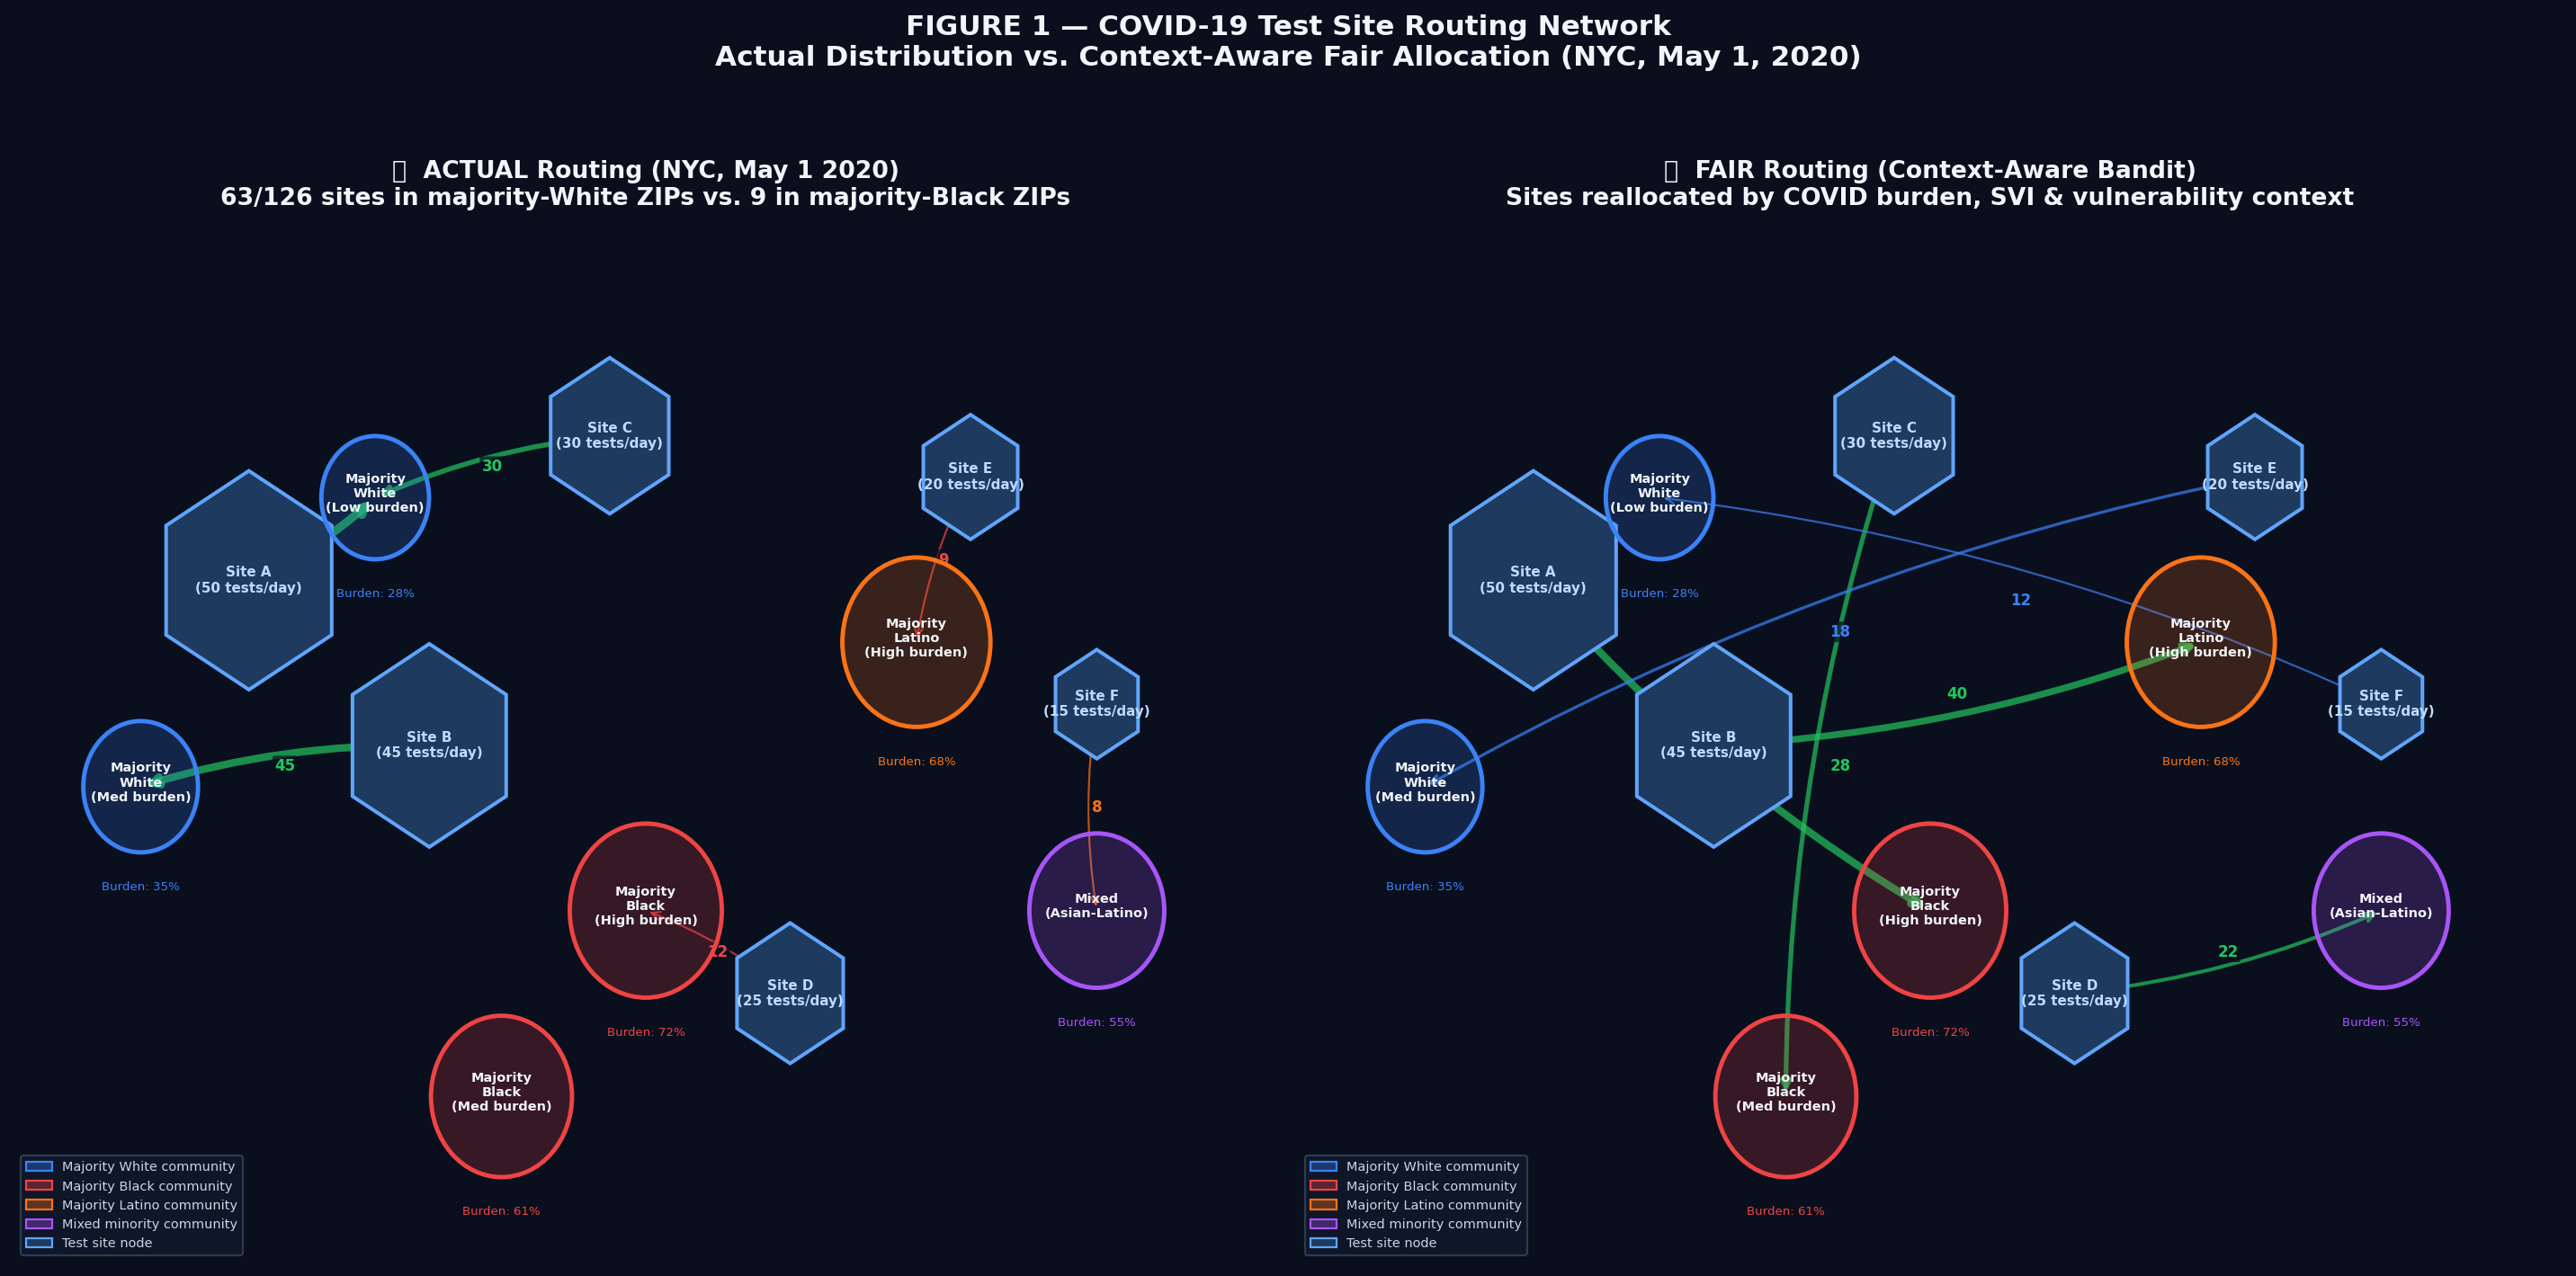
\includegraphics[width=\textwidth,height=0.66\textheight,keepaspectratio]{../analysis_artifacts/fig1_routing_network.png}}{%
\IfFileExists{../analysis_artifacts/graph1_routing.png}{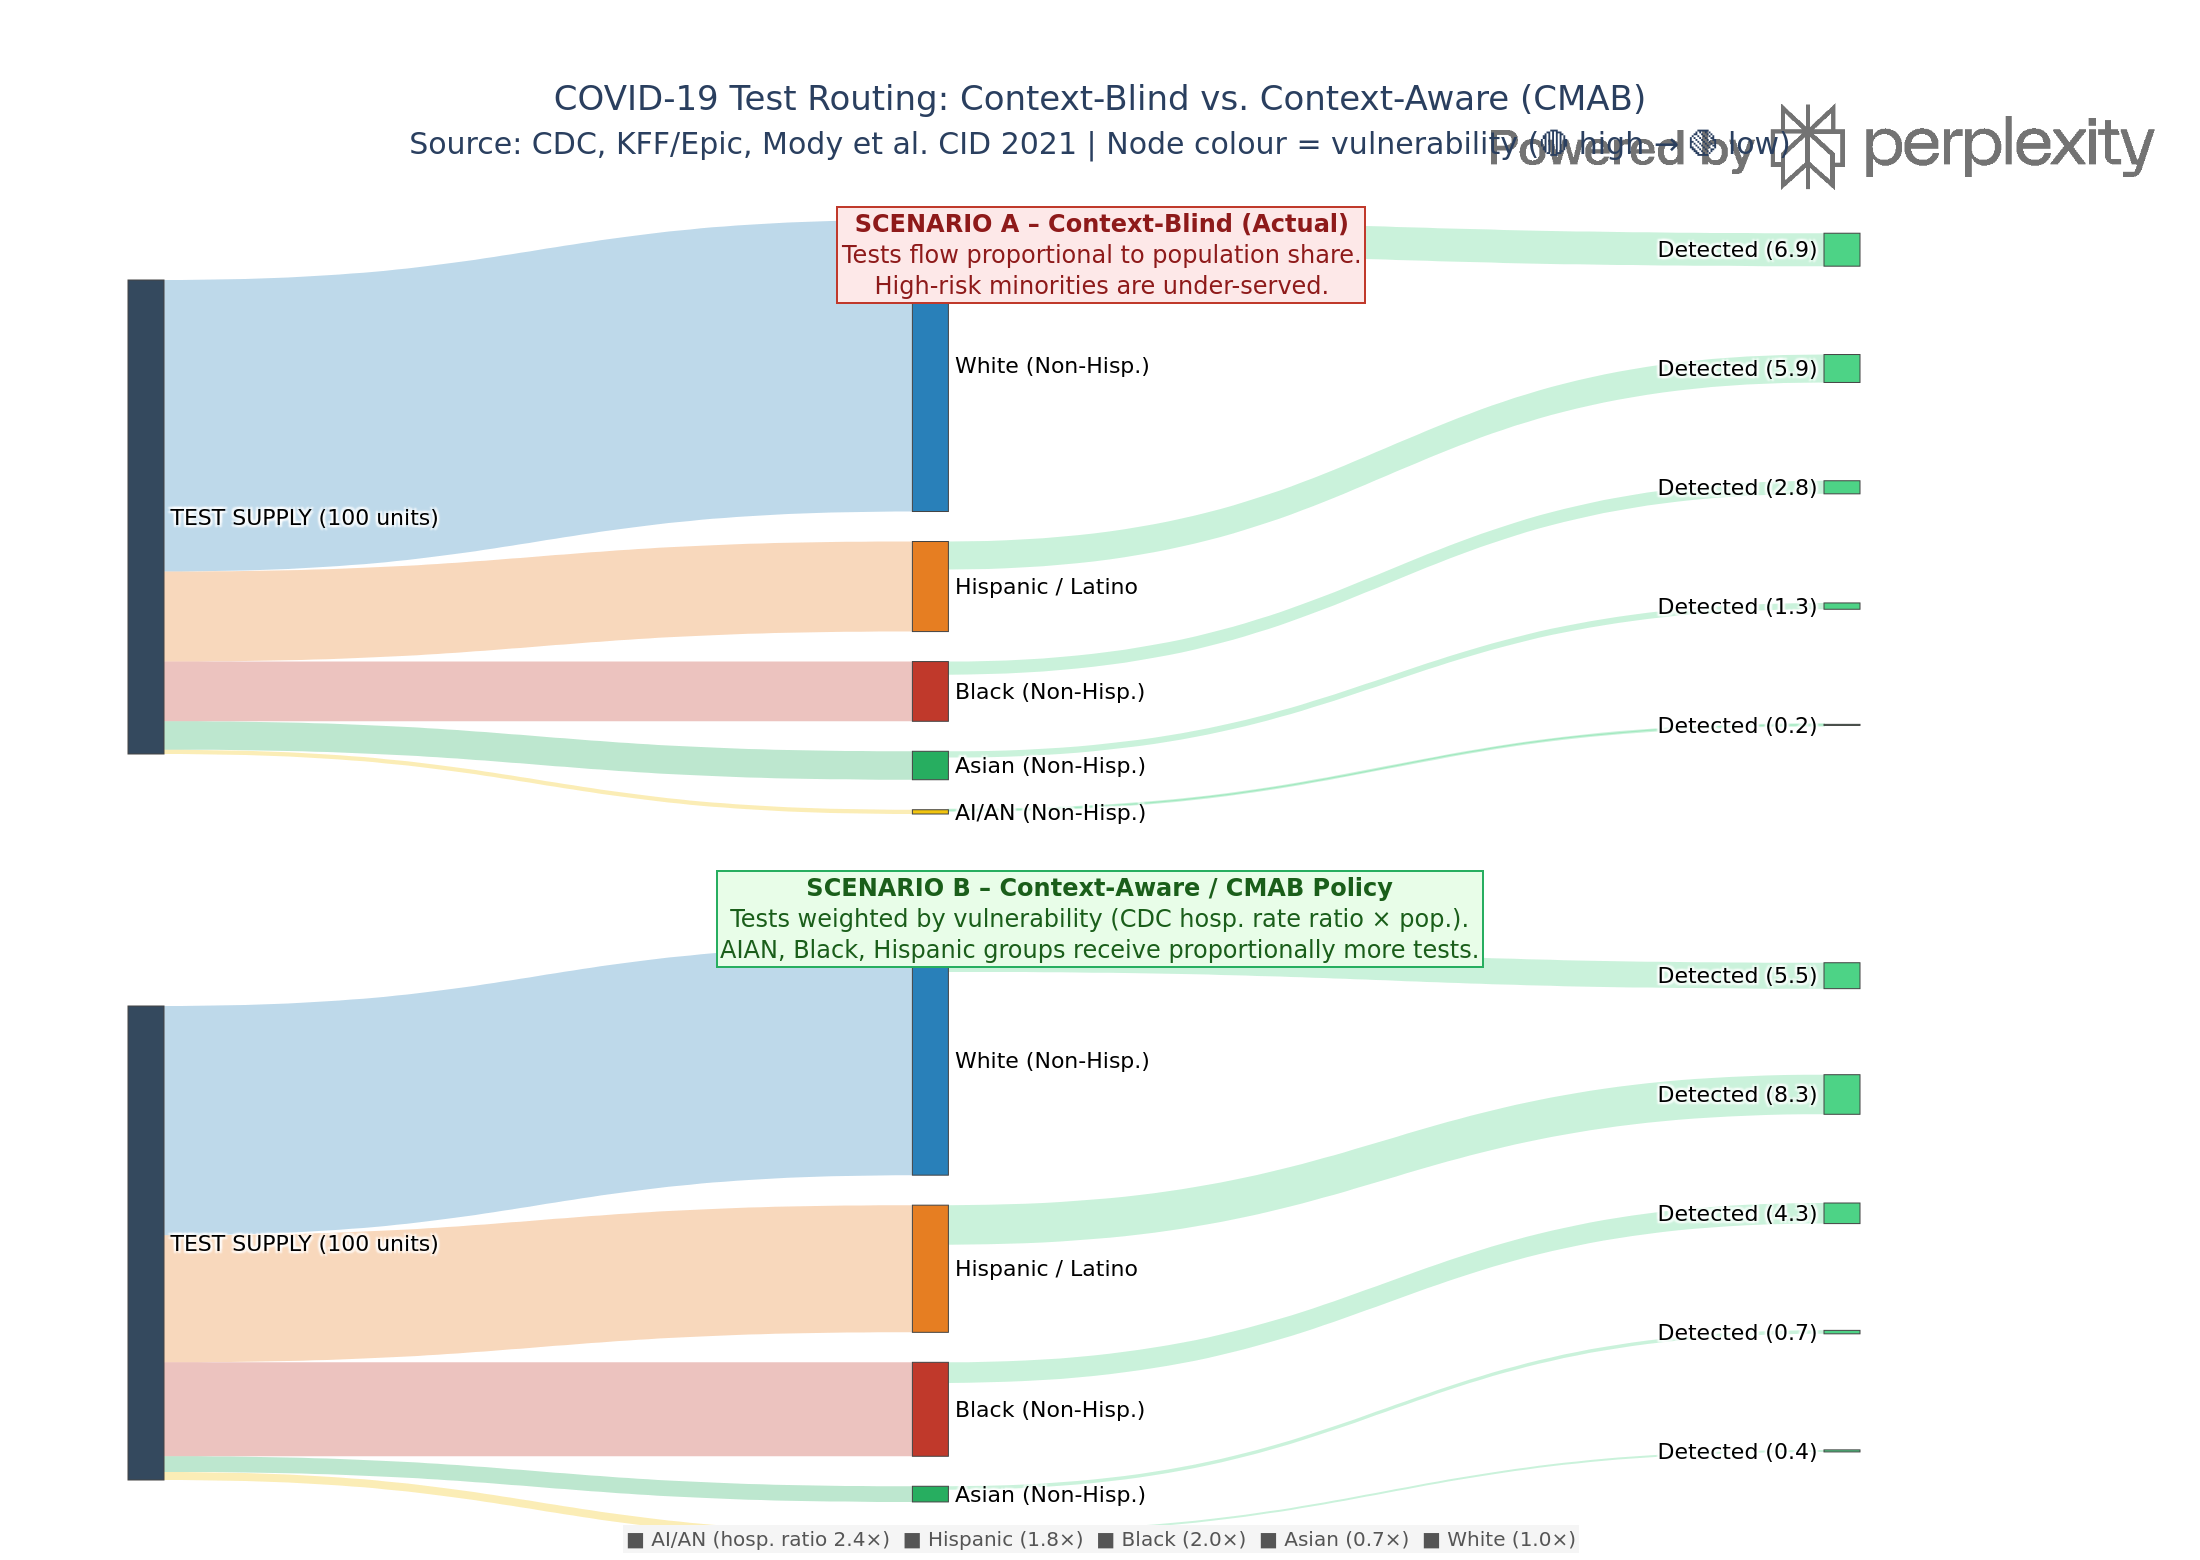
\includegraphics[width=\textwidth,height=0.66\textheight,keepaspectratio]{../analysis_artifacts/graph1_routing.png}}{%
\IfFileExists{../analysis_artifacts/graph1_context_blind_vs_cmab.png}{\includegraphics[width=\textwidth,height=0.66\textheight,keepaspectratio]{../analysis_artifacts/graph1_context_blind_vs_cmab.png}}{%
\IfFileExists{../analysis_artifacts/inefficient_test_routing.png}{\includegraphics[width=\textwidth,height=0.66\textheight,keepaspectratio]{../analysis_artifacts/inefficient_test_routing.png}}{%
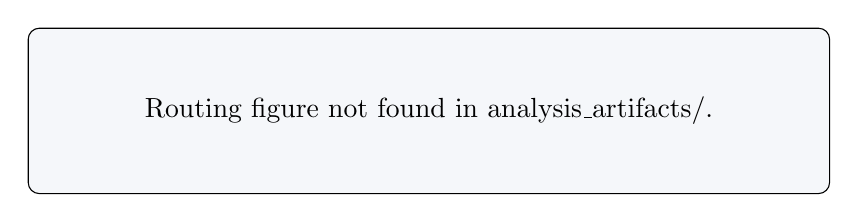
\begin{tikzpicture}\node[draw,rounded corners,fill=softgray,text width=0.82\textwidth,align=center,minimum height=2.1cm]{Routing figure not found in analysis\_artifacts/.};\end{tikzpicture}}}}}}

\newcommand{\diagnosticfig}{%
\IfFileExists{../analysis_artifacts/fig2_trial_bias.png}{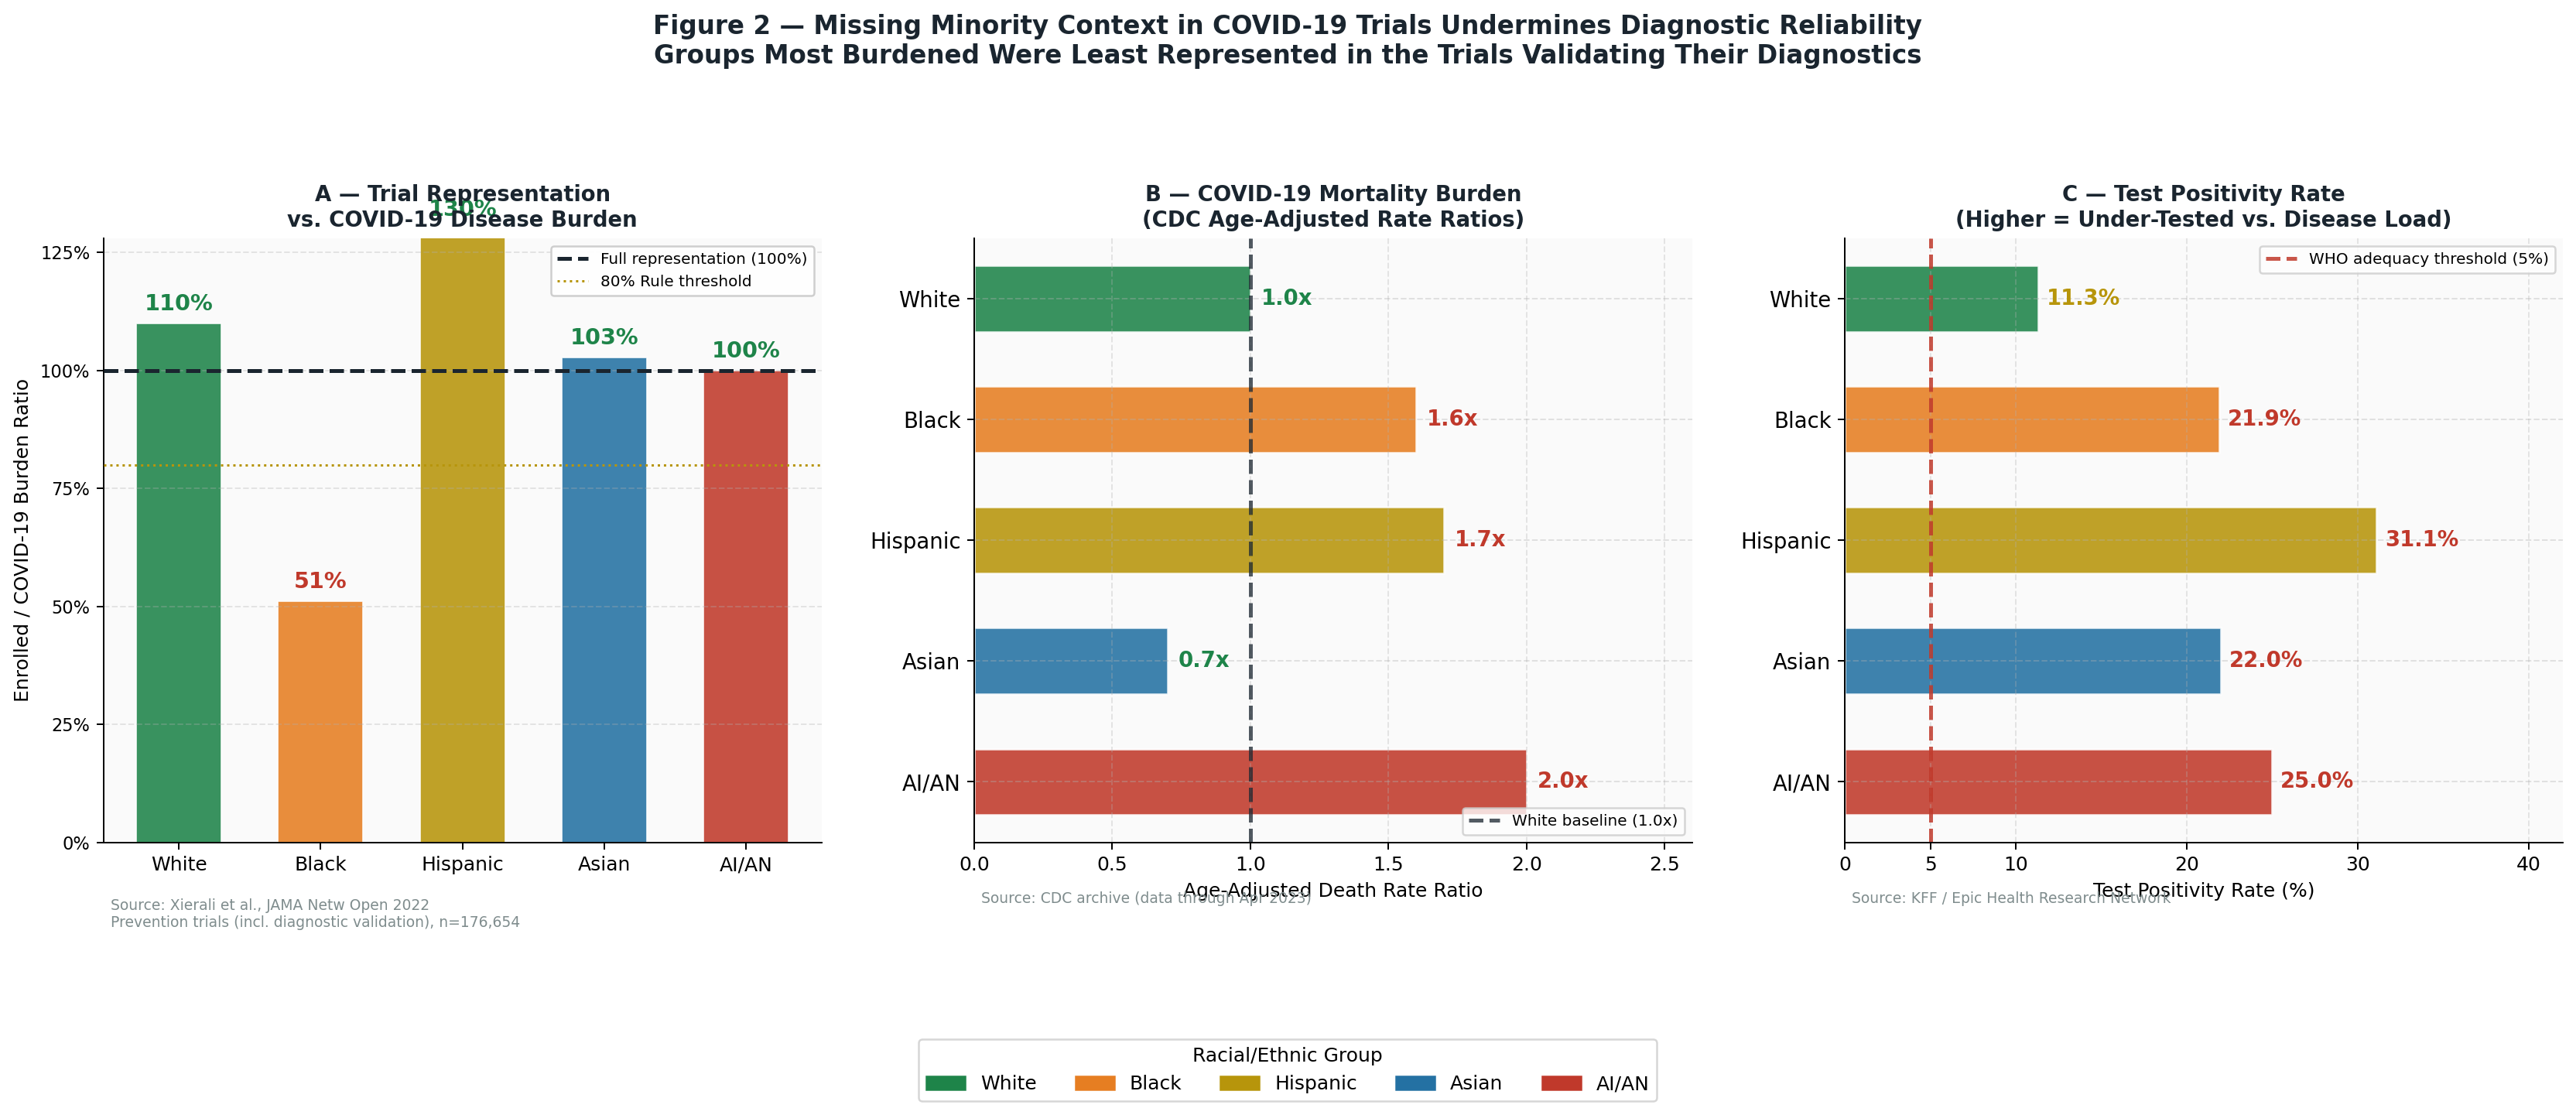
\includegraphics[width=\textwidth,height=0.66\textheight,keepaspectratio]{../analysis_artifacts/fig2_trial_bias.png}}{%
\IfFileExists{../analysis_artifacts/graph2_trial_bias.png}{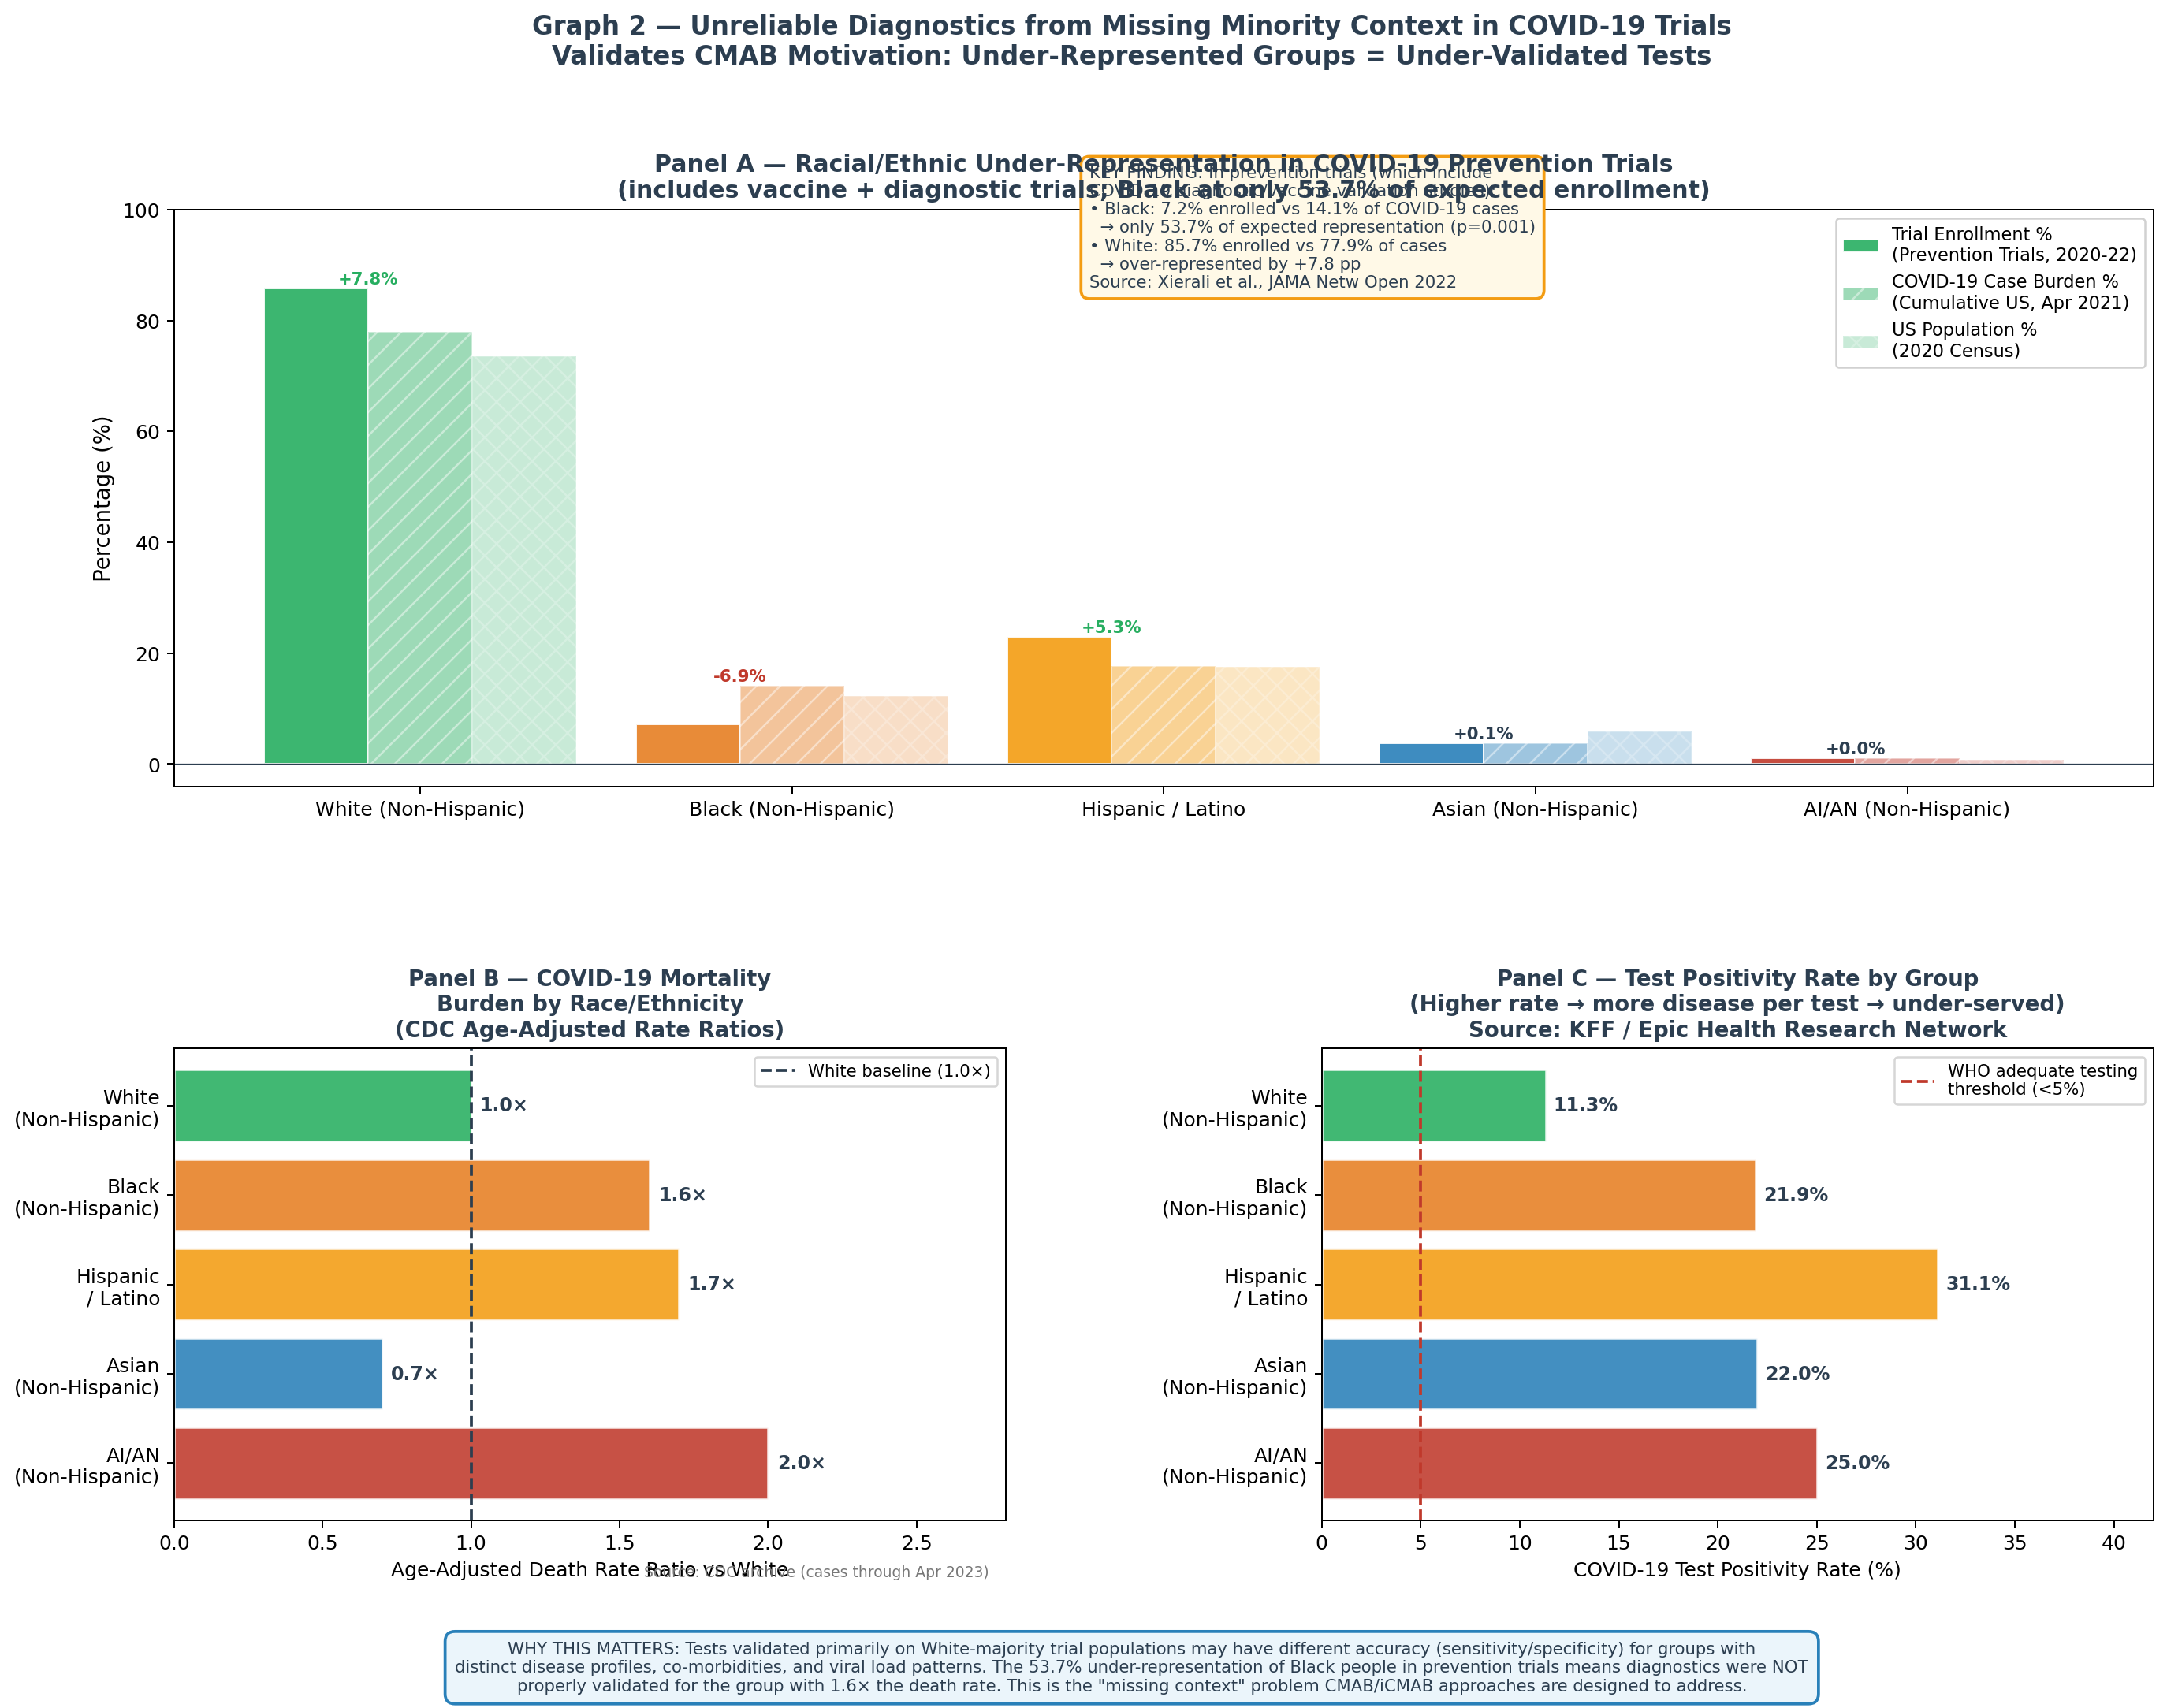
\includegraphics[width=\textwidth,height=0.66\textheight,keepaspectratio]{../analysis_artifacts/graph2_trial_bias.png}}{%
\IfFileExists{../analysis_artifacts/graph2_unreliable_diagnostics.png}{\includegraphics[width=\textwidth,height=0.66\textheight,keepaspectratio]{../analysis_artifacts/graph2_unreliable_diagnostics.png}}{%
\IfFileExists{../analysis_artifacts/unreliable_diagnostics_missing_context.png}{\includegraphics[width=\textwidth,height=0.66\textheight,keepaspectratio]{../analysis_artifacts/unreliable_diagnostics_missing_context.png}}{%
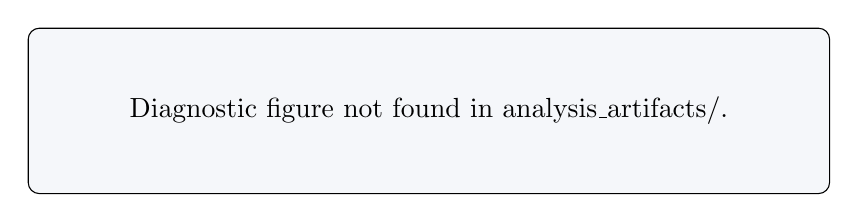
\begin{tikzpicture}\node[draw,rounded corners,fill=softgray,text width=0.82\textwidth,align=center,minimum height=2.1cm]{Diagnostic figure not found in analysis\_artifacts/.};\end{tikzpicture}}}}}}

\newcommand{\confusionfig}{%
\IfFileExists{../analysis_artifacts/fig3_confusion_matrices.png}{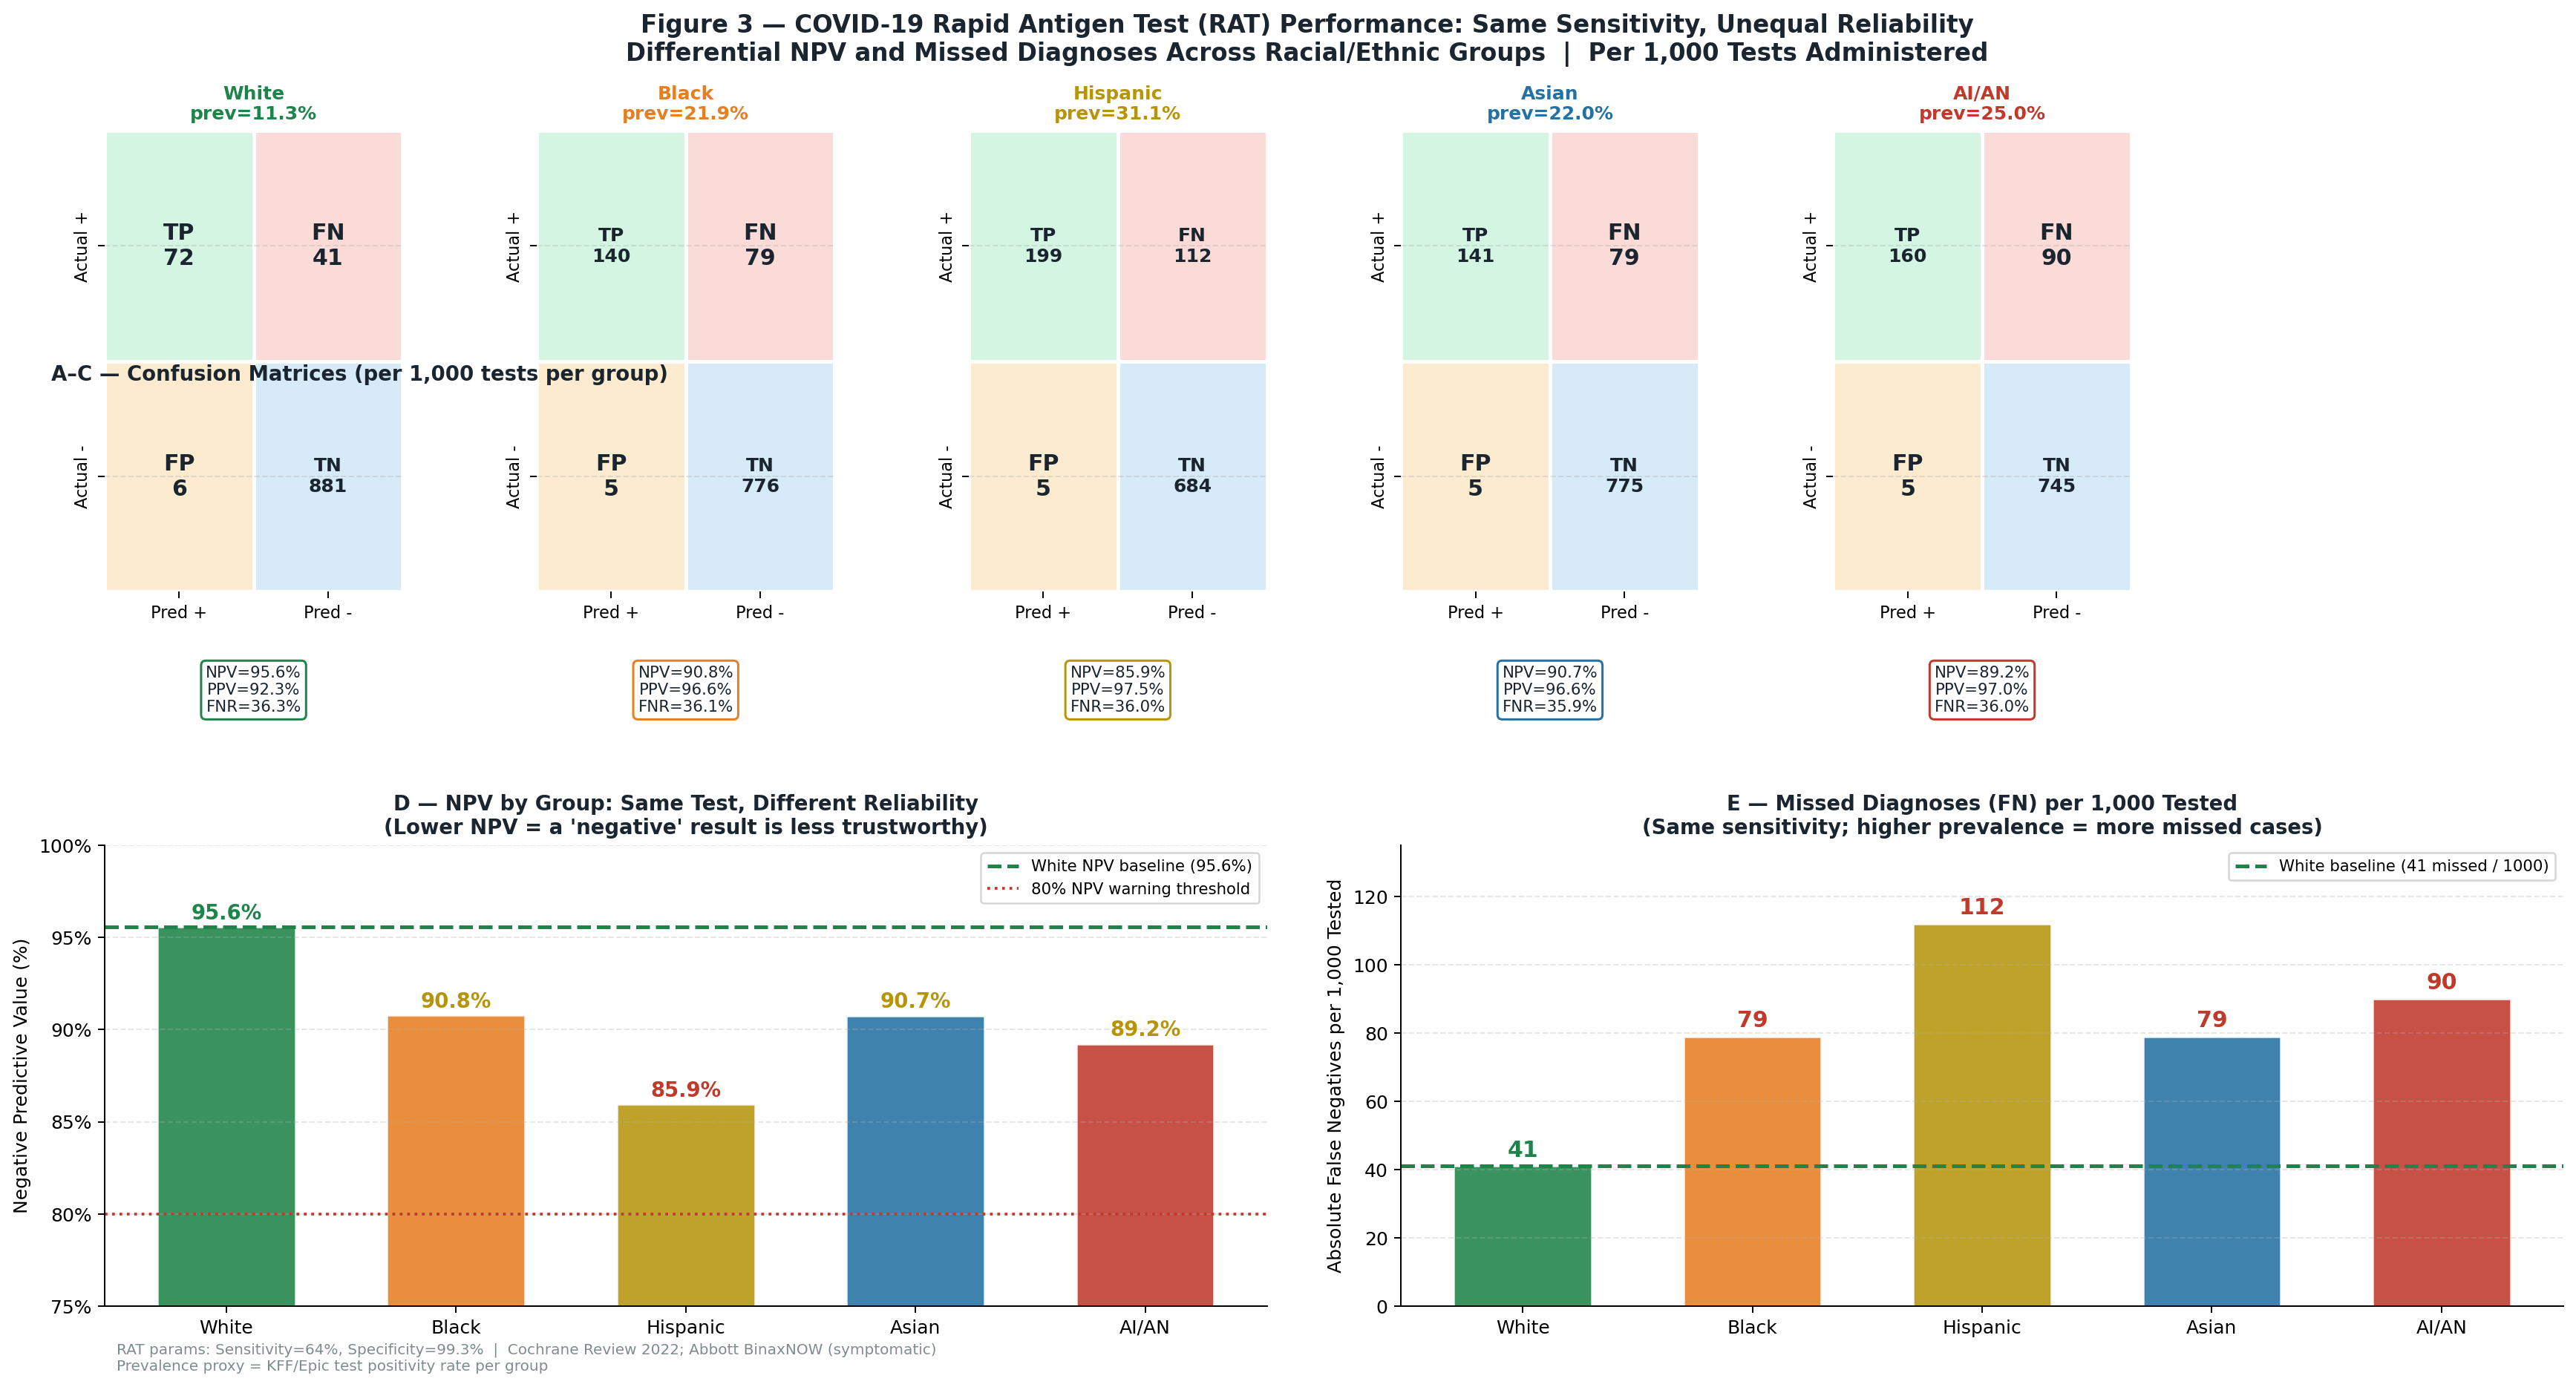
\includegraphics[width=\textwidth,height=0.66\textheight,keepaspectratio]{../analysis_artifacts/fig3_confusion_matrices.png}}{%
\IfFileExists{../analysis_artifacts/graph3_confusion_matrices.png}{\includegraphics[width=\textwidth,height=0.66\textheight,keepaspectratio]{../analysis_artifacts/graph3_confusion_matrices.png}}{%
\IfFileExists{../analysis_artifacts/graph3_confusion_matrix_routing.png}{\includegraphics[width=\textwidth,height=0.66\textheight,keepaspectratio]{../analysis_artifacts/graph3_confusion_matrix_routing.png}}{%
\IfFileExists{../analysis_artifacts/graph4_confusion_matrix_diagnostics.png}{\includegraphics[width=\textwidth,height=0.66\textheight,keepaspectratio]{../analysis_artifacts/graph4_confusion_matrix_diagnostics.png}}{%
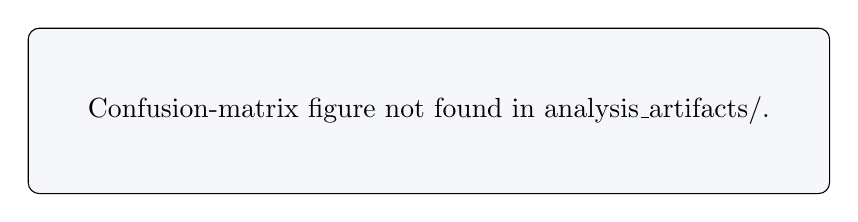
\begin{tikzpicture}\node[draw,rounded corners,fill=softgray,text width=0.82\textwidth,align=center,minimum height=2.1cm]{Confusion-matrix figure not found in analysis\_artifacts/.};\end{tikzpicture}}}}}}

\begin{document}

\begin{frame}
  \titlepage
\end{frame}

\begin{frame}{Project Overview}
\begin{block}{What this project is}
This project studies \textbf{fairness-aware routing under missing context} in two environment families:
\textbf{clinical decision support} and \textbf{quantum-network routing}.
\end{block}

\vspace{0.5em}

\begin{block}{Shared problem}
Both domains are \textbf{sequential decision systems (SDSs)}:
they allocate scarce resources under uncertainty, observe only partial feedback,
and update future decisions from incomplete evidence.
\end{block}

\vspace{0.5em}

\textbf{Project goals}
\begin{itemize}
    \item Compare \mab, \cmab, and \icmab{} strategies.
    \item Measure both \textbf{performance} and \textbf{fairness}.
    \item Show how missing or degraded context can create repeated allocation harm.
    \item Build a reproducible framework with reportable artifacts.
\end{itemize}
\end{frame}


\begin{frame}{Why This Project Matters}
\begin{columns}[T]
\begin{column}{0.48\textwidth}
\begin{block}{Clinical impact}
Routing decisions affect real patient outcomes.
\end{block}

\begin{itemize}
    \item Who receives a diagnostic test?
    \item Who gets retested or escalated?
    \item Whose risk is missed because context is incomplete?
\end{itemize}

\vspace{0.4em}

\alert{A policy can look accurate on average while still delaying access to critical resources/care for a vulnerable group.}
\end{column}

\begin{column}{0.48\textwidth}
\begin{block}{Quantum-network impact}
Routing decisions affect service quality under noisy conditions.
\end{block}

\begin{itemize}
    \item Which path gets selected?
    \item Which flows receive scarce qubit or link resources?
    \item Which users experience repeated failure or latency?
\end{itemize}

\vspace{0.4em}

\alert{A policy can maximize total throughput while still giving some flows consistently worse service.}
\end{column}
\end{columns}

\vspace{0.6em}

\begin{block}{Core reason this matters}
Fairness-aware routing asks whether the system is making good decisions
\textbf{for everyone affected}, not only good decisions on average.
\end{block}
\end{frame}


\begin{frame}{Updated Domain Model}
\centering
\resizebox{0.90\textwidth}{!}{%
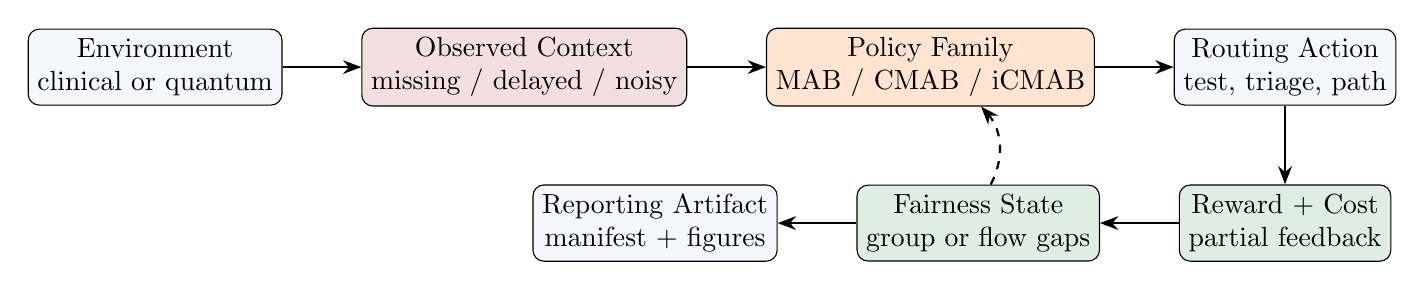
\begin{tikzpicture}[
  node distance=0.7cm,
  entity/.style={draw, rounded corners, align=center, fill=softgray, minimum width=2.5cm, minimum height=0.8cm},
  risk/.style={draw, rounded corners, align=center, fill=softred!18, minimum width=2.5cm, minimum height=0.8cm},
  decision/.style={draw, rounded corners, align=center, fill=ritorange!18, minimum width=2.5cm, minimum height=0.8cm},
  output/.style={draw, rounded corners, align=center, fill=softgreen!18, minimum width=2.5cm, minimum height=0.8cm},
  arr/.style={-{Stealth}, thick}
]
\node[entity] (env) {Environment\\clinical or quantum};
\node[risk, right=1.0cm of env] (ctx) {Observed Context\\missing / delayed / noisy};
\node[decision, right=1.0cm of ctx] (pol) {Policy Family\\MAB / CMAB / iCMAB};
\node[entity, right=1.0cm of pol] (act) {Routing Action\\test, triage, path};
\node[output, below=1.0cm of act] (reward) {Reward + Cost\\partial feedback};
\node[output, left=1.0cm of reward] (fair) {Fairness State\\group or flow gaps};
\node[entity, left=1.0cm of fair] (report) {Reporting Artifact\\manifest + figures};

\draw[arr] (env) -- (ctx);
\draw[arr] (ctx) -- (pol);
\draw[arr] (pol) -- (act);
\draw[arr] (act) -- (reward);
\draw[arr] (reward) -- (fair);
\draw[arr] (fair) -- (report);
\draw[arr,dashed] (fair) to[bend right=35] (pol);
\end{tikzpicture}}

\vspace{0.55em}
\scriptsize
\begin{tabular}{p{0.24\textwidth}p{0.58\textwidth}p{0.12\textwidth}}
\toprule
\textbf{Relationship} & \textbf{Meaning} & \textbf{Cardinality} \\
\midrule
Environment $\rightarrow$ Context & each run produces observed context snapshots & 1 to 1..* \\
Context $\rightarrow$ Policy & one observed state is used for the current decision & 1 to 1 \\
Policy $\rightarrow$ Action & the policy selects exactly one routing action & 1 to 1 \\
Action $\rightarrow$ Outcome & only the chosen action creates observed feedback & 1 to 1 \\
Outcome $\rightarrow$ Fairness & outcomes update fairness metrics over groups or routes & 1 to 1..* \\
Fairness $\rightarrow$ Report & validation stores summaries, figures, and manifests & 1 to 0..* \\
\bottomrule
\end{tabular}

\vspace{0.35em}
\begin{itemize}
  \item The same domain model supports both environment families.
  \item The unchosen actions remain \textbf{counterfactual}; only the chosen action produces observed feedback.
  \item Fairness risk appears when context quality is systematically worse for one group, site, cohort, or route class.
\end{itemize}
\end{frame}

\begin{frame}{Why the Domain Model Changed}
\begin{columns}[T]
\begin{column}{0.48\textwidth}
\centering
\textbf{Old domain view}

\vspace{0.3em}
\resizebox{\linewidth}{!}{%
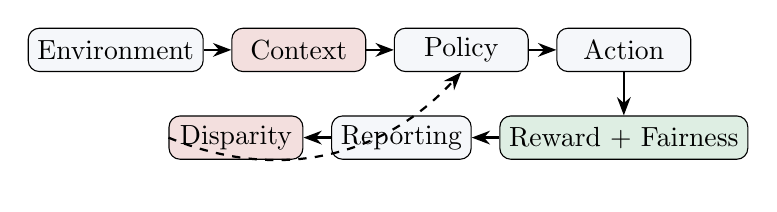
\begin{tikzpicture}[
  node distance=0.42cm,
  smallbox/.style={draw, rounded corners, align=center, minimum width=1.7cm, minimum height=0.55cm, fill=softgray},
  bad/.style={draw, rounded corners, align=center, minimum width=1.7cm, minimum height=0.55cm, fill=softred!18},
  good/.style={draw, rounded corners, align=center, minimum width=1.7cm, minimum height=0.55cm, fill=softgreen!18},
  arr/.style={-{Stealth}, thick}
]
\node[smallbox] (env) {Environment};
\node[bad, right=0.35cm of env] (ctx) {Context};
\node[smallbox, right=0.35cm of ctx] (pol) {Policy};
\node[smallbox, right=0.35cm of pol] (act) {Action};
\node[good, below=0.55cm of act] (out) {Reward + Fairness};
\node[smallbox, left=0.35cm of out] (rep) {Reporting};
\node[bad, left=0.35cm of rep] (harm) {Disparity};

\draw[arr] (env) -- (ctx);
\draw[arr] (ctx) -- (pol);
\draw[arr] (pol) -- (act);
\draw[arr] (act) -- (out);
\draw[arr] (out) -- (rep);
\draw[arr] (rep) -- (harm);
\draw[arr,dashed] (harm.west) to[bend right=35] (pol.south);
\end{tikzpicture}}
\vspace{0.35em}

{\scriptsize Compact pipeline, but some concepts were merged together.}
\end{column}

\begin{column}{0.48\textwidth}
\centering
\textbf{Updated domain view}

\vspace{0.3em}
\resizebox{\linewidth}{!}{%
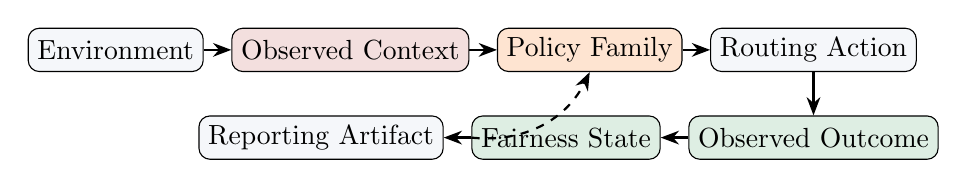
\begin{tikzpicture}[
  node distance=0.42cm,
  smallbox/.style={draw, rounded corners, align=center, minimum width=1.7cm, minimum height=0.55cm, fill=softgray},
  bad/.style={draw, rounded corners, align=center, minimum width=1.7cm, minimum height=0.55cm, fill=softred!18},
  good/.style={draw, rounded corners, align=center, minimum width=1.7cm, minimum height=0.55cm, fill=softgreen!18},
  orangebox/.style={draw, rounded corners, align=center, minimum width=1.7cm, minimum height=0.55cm, fill=ritorange!18},
  arr/.style={-{Stealth}, thick}
]
\node[smallbox] (env) {Environment};
\node[bad, right=0.35cm of env] (ctx) {Observed Context};
\node[orangebox, right=0.35cm of ctx] (pol) {Policy Family};
\node[smallbox, right=0.35cm of pol] (act) {Routing Action};
\node[good, below=0.55cm of act] (out) {Observed Outcome};
\node[good, left=0.35cm of out] (fair) {Fairness State};
\node[smallbox, left=0.35cm of fair] (rep) {Reporting Artifact};

\draw[arr] (env) -- (ctx);
\draw[arr] (ctx) -- (pol);
\draw[arr] (pol) -- (act);
\draw[arr] (act) -- (out);
\draw[arr] (out) -- (fair);
\draw[arr] (fair) -- (rep);
\draw[arr,dashed] (fair.west) to[bend right=35] (pol.south);
\end{tikzpicture}}
\vspace{0.35em}

{\scriptsize Clearer separation of decision, outcome, fairness audit, and reporting.}
\end{column}
\end{columns}

\vspace{0.6em}
\begin{block}{Why this matters}
\begin{itemize}
    \item The updated model separates \textbf{observed outcome} from \textbf{fairness state}, so fairness is treated as an audit layer rather than being hidden inside reward.
    \item It makes the \textbf{bandit setting} clearer: only the chosen action is observed, while the other actions remain \textbf{counterfactual}.
    \item It also makes the project more reproducible by showing that \textbf{reporting/validation artifacts} are explicit outputs of the framework.
\end{itemize}
\end{block}
\end{frame}

\begin{frame}{Best Evidence Figure 1: Test Routing Failure vs. Context-Aware Routing}
\begin{center}
\routingfig
\end{center}
\vspace{-0.3em}
\small \textbf{Finding:} context-blind routing detects \textbf{17.2 cases per 100 tests}, while context-aware \cmab routing detects \textbf{19.3 cases per 100 tests}, a \textbf{12.5\% efficiency gain} while increasing allocation to AIAN, Black, and Hispanic groups.
\end{frame}

\begin{frame}{Best Evidence Figure 2: Missing Minority Context in Diagnostics}
\begin{center}
\diagnosticfig
\end{center}
\vspace{-0.3em}
\small \textbf{Finding:} groups with higher COVID mortality and positivity were also less represented in diagnostic-validation evidence; Black participants appear at \textbf{53.7\% of expected representation} in prevention/diagnostic trials.
\end{frame}

\begin{frame}{Best Evidence Figure 3: Confusion-Matrix Reliability Gaps}
\begin{center}
\confusionfig
\end{center}
\vspace{-0.3em}
\small \textbf{Finding:} the same diagnostic policy can produce different false-negative and NPV behavior across groups when prevalence and validation representation differ.
\end{frame}

\begin{frame}{Updated Architecture Overview}
\begin{center}
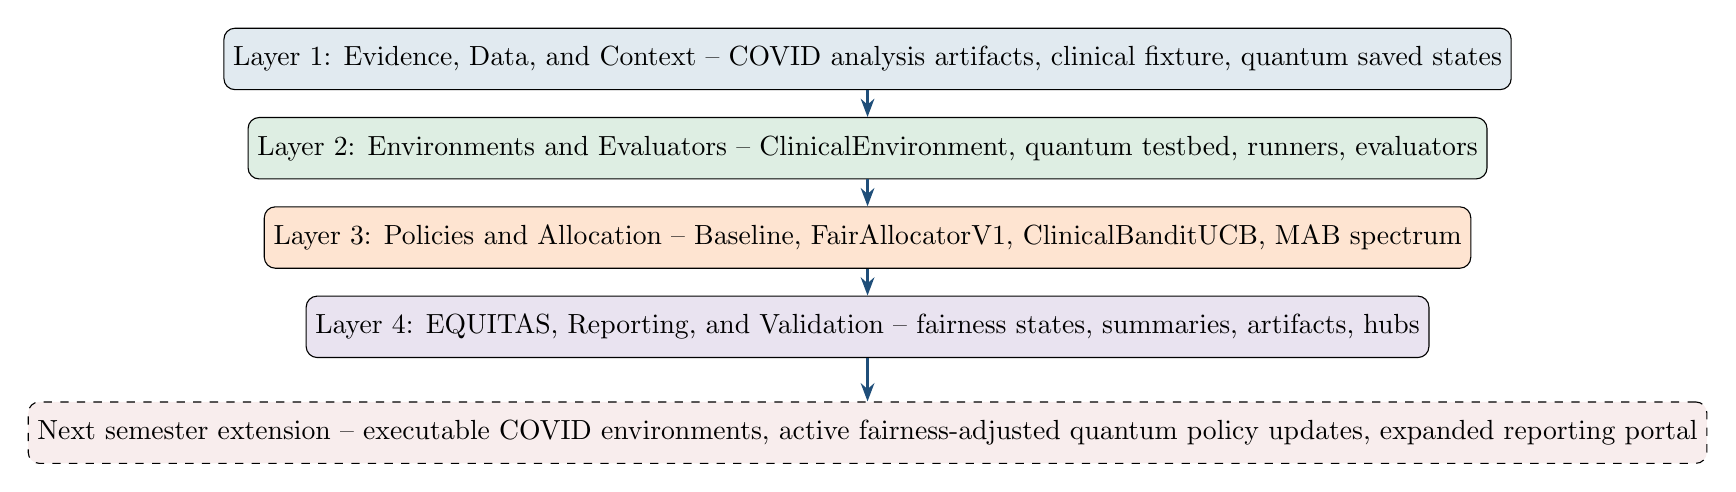
\begin{tikzpicture}[
  layer/.style={draw, rounded corners, align=center, minimum width=10.4cm, minimum height=0.78cm, fill=softgray},
  future/.style={draw, dashed, rounded corners, align=center, minimum width=10.4cm, minimum height=0.78cm, fill=softred!10},
  arr/.style={-{Stealth}, thick, deepblue}
]
\node[layer, fill=softblue!18] (data) {Layer 1: Evidence, Data, and Context -- COVID analysis artifacts, clinical fixture, quantum saved states};
\node[layer, fill=softgreen!18, below=0.34cm of data] (env) {Layer 2: Environments and Evaluators -- ClinicalEnvironment, quantum testbed, runners, evaluators};
\node[layer, fill=ritorange!18, below=0.34cm of env] (policy) {Layer 3: Policies and Allocation -- Baseline, FairAllocatorV1, ClinicalBanditUCB, MAB spectrum};
\node[layer, fill=softpurple!18, below=0.34cm of policy] (report) {Layer 4: EQUITAS, Reporting, and Validation -- fairness states, summaries, artifacts, hubs};
\node[future, below=0.55cm of report] (future) {Next semester extension -- executable COVID environments, active fairness-adjusted quantum policy updates, expanded reporting portal};
\draw[arr] (data) -- (env);
\draw[arr] (env) -- (policy);
\draw[arr] (policy) -- (report);
\draw[arr] (report) -- (future);
\end{tikzpicture}
\end{center}
\vspace{0.35em}
\begin{block}{Implementation stack}
\textbf{Python} for environments and evaluation, \textbf{Jupyter notebooks} for reproducibility and demo, \textbf{GitHub / Actions} for versioning and smoke validation, and \textbf{LaTeX} for report-ready outputs.
\end{block}
\end{frame}

\begin{frame}{Architecture Layer 1: Evidence, Data, and Context}
\begin{columns}[T]
\begin{column}{0.48\textwidth}
\textbf{Inputs}
\begin{itemize}
    \item COVID clinical evidence artifacts
    \item clinical synthetic fixture
    \item EQUITAS context fields
    \item quantum legacy saved states
\end{itemize}

\textbf{Key fields}
\begin{itemize}
    \item group, site, cohort, service line
    \item test distribution, escalation action
    \item reward, success, latency
    \item route choice, allocator, evaluator state
\end{itemize}
\end{column}
\begin{column}{0.48\textwidth}
\begin{block}{Layer role}
This layer converts raw evidence into the structured context that every later layer depends on.
\end{block}
\begin{block}{Why this layer matters}
The new analysis artifacts make the clinical side evidence-based: vulnerability, representation, and measurement quality must be modeled before a fair policy can act.
\end{block}
\end{column}
\end{columns}
\end{frame}

\begin{frame}{Architecture Layer 2: Environments and Evaluators}
\begin{columns}[T]
\begin{column}{0.47\textwidth}
\textbf{Clinical path}
\begin{itemize}
    \item \texttt{ClinicalEnvironment}
    \item \texttt{ClinicalExperimentRunner}
    \item \texttt{ClinicalExperimentEvaluator}
    \item embedded clinical allocation fixture
\end{itemize}
\vspace{0.4em}
\textbf{Quantum path}
\begin{itemize}
    \item quantum-routing testbeds
    \item evaluator + saved-state conventions
    \item fairness sidecar compatibility path
\end{itemize}
\end{column}
\begin{column}{0.49\textwidth}
\begin{center}
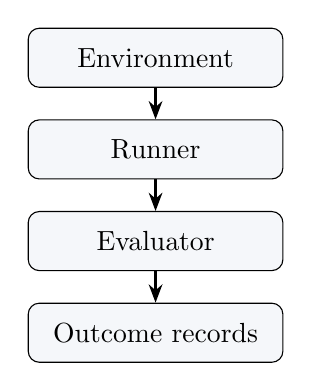
\begin{tikzpicture}[
cls/.style={draw,rounded corners,fill=softgray,align=center,text width=3.0cm,minimum height=0.75cm},
arr/.style={-{Stealth},thick}
]
\node[cls] (e) {Environment};
\node[cls, below=0.4cm of e] (r) {Runner};
\node[cls, below=0.4cm of r] (v) {Evaluator};
\node[cls, below=0.4cm of v] (o) {Outcome records};
\draw[arr] (e) -- (r);
\draw[arr] (r) -- (v);
\draw[arr] (v) -- (o);
\end{tikzpicture}
\end{center}
\begin{block}{Layer relationship}
The evaluator standardizes outcome records so clinical and quantum runs can be compared through the same reporting surface.
\end{block}
\end{column}
\end{columns}
\end{frame}

\begin{frame}{Architecture Layer 3: Policies and Allocation}
\begin{center}
\begin{tabular}{p{0.19\textwidth}p{0.23\textwidth}p{0.25\textwidth}p{0.23\textwidth}}
\toprule
Family & Decision signal & Strength & Main fairness risk \\
\midrule
\mab & action history & simple baseline & repeats historical allocation patterns \\
\cmab & observed context & better utility & inherits incomplete or biased context \\
\icmab & context + mediated state & richer adaptation & depends on quality of fairness mediation \\
\bottomrule
\end{tabular}
\end{center}

\vspace{0.5em}
\begin{block}{Clinical model families already running}
\texttt{Oracle}, \texttt{ClinicalBaseline}, \texttt{FairAllocatorV1}, and \texttt{ClinicalBanditUCB}.
\end{block}
\begin{equation*}
\text{decision}_t = \arg\max_a \left[\text{utility}_{t,a} - \lambda \cdot \text{expected disparity}_{t,a}\right]
\end{equation*}
\small This captures the main idea: the chosen action balances utility against anticipated disparity.
\end{frame}

\begin{frame}{Architecture Layer 4: EQUITAS, Reporting, and Validation}
\begin{columns}[T]
\begin{column}{0.48\textwidth}
\textbf{EQUITAS mediation}
\begin{itemize}
    \item attaches audit / mitigation context
    \item tracks group-conditioned outcomes
    \item preserves fields needed for fairness analysis
    \item supports stratified summaries by model and group
\end{itemize}
\end{column}
\begin{column}{0.48\textwidth}
\textbf{Reporting and validation}
\begin{itemize}
    \item fairness manifests and sidecar artifacts
    \item model-stratified fairness summaries
    \item validation hubs linking figures/tables to evidence
    \item notebook-facing reproducibility workflow
\end{itemize}
\end{column}
\end{columns}
\vspace{0.45em}
\begin{block}{Current validation snapshot}
The clinical fairness smoke produced \textbf{16 fairness states}; reporting produced \textbf{21 manifest-linked artifacts}; the quantum legacy path remains compatible with fairness sidecars.
\end{block}
\end{frame}

\begin{frame}{Preliminary Results Snapshot}
\begin{center}
\begin{tabular}{p{0.42\textwidth}p{0.44\textwidth}}
\toprule
Evidence item & Result \\
\midrule
Clinical embedded path & evaluator, runner, environment, allocator, models, and EQUITAS context run end-to-end \\
Clinical fairness smoke & 16 fairness states across four model families \\
Non-oracle efficiency & FairAllocatorV1: 91.23\%; ClinicalBanditUCB: 84.21\%; ClinicalBaseline: 75.09\% oracle efficiency \\
Reporting layer & 21 manifest-linked artifacts and model-stratified summaries \\
Quantum compatibility & legacy quantum path preserved with fairness sidecar artifacts \\
\bottomrule
\end{tabular}
\end{center}
\vspace{0.35em}
\begin{block}{Interpretation}
The framework already supports reproducible cross-domain fairness evaluation. Claims about active fairness-adjusted quantum learning still require an explicit policy-update mechanism and full validation.
\end{block}
\end{frame}

\begin{frame}{GitHub Code Review Break}
\begin{block}{What I will show live on GitHub}
Open the repository and connect each class to the architecture diagram.
\end{block}
\begin{center}
\small
\begin{tabular}{p{0.34\textwidth}p{0.49\textwidth}}
\toprule
Class / file to show & Architecture connection \\
\midrule
\texttt{ClinicalExperimentEvaluator} & Layer 2 evaluator orchestration and artifact capture \\
\texttt{ClinicalExperimentRunner} & Layer 2 run execution over seeds, models, and allocations \\
\texttt{FairAllocatorV1} or \texttt{ClinicalBanditUCB} & Layer 3 policy and allocation decision logic \\
\texttt{equitas\_mediator.py} & Layer 4 fairness audit and mitigation context \\
\bottomrule
\end{tabular}
\end{center}
\vspace{0.4em}
\small Emphasize readable formatting, comments, class responsibility, and how the code mirrors the layered architecture.
\end{frame}

\begin{frame}{What I Will Complete Next Semester}
\begin{enumerate}
    \item Convert the COVID test-allocation and diagnostic-bias analyses into fully executable clinical environments.
    \item Add the strongest analysis artifacts into the final paper and reporting pipeline.
    \item Complete active fairness-adjusted quantum policy updates.
    \item Split validation into dedicated \textbf{efficiency} and \textbf{fairness} hubs.
    \item Build a richer reporting portal for experiments, validation, and paper-ready evidence.
\end{enumerate}
\vspace{0.5em}
\begin{block}{Architecture view}
These next steps mainly extend Layer 1 (data/context), Layer 3 (fairness-aware policies), and Layer 4 (reporting and validation).
\end{block}
\end{frame}

\begin{frame}{Working Demo Plan}
\begin{enumerate}
    \item Run the clinical fairness demo or smoke-validation notebook.
    \item Show generated fairness states and model-stratified summaries.
    \item Show report artifacts and manifest linkage.
    \item Open the validation hub and connect the figures to the evidence claims.
    \item Show where the new COVID clinical artifacts fit into the next-semester executable environments.
\end{enumerate}
\vspace{0.5em}
\begin{block}{Demo objective}
Show that the system runs, records fairness evidence, and produces artifacts directly connected to the domain model and architecture.
\end{block}
\end{frame}

\begin{frame}{Takeaway}
\begin{block}{Main claim}
Context quality is a fairness variable. Missing, ignored, or biased context can turn partial-feedback learning into repeated allocation harm.
\end{block}
\begin{block}{What was built}
A clinical--quantum evaluation framework that compares performance and fairness across the selected MAB spectrum while preserving reproducible artifacts.
\end{block}
\begin{block}{What the new analysis adds}
The new clinical figures validate the missing-context harm model: test routing improved under context-aware allocation, and diagnostic reliability changed when group context was missing or under-represented.
\end{block}
\end{frame}

\begin{frame}[allowframebreaks]{Selected References}
\scriptsize
\begin{thebibliography}{99}
\bibitem{kffepic} KFF/Epic. COVID-19 racial disparities in testing, infection, hospitalization, and death.
\bibitem{cdcdisparities} CDC. Risk for COVID-19 infection, hospitalization, and death by race/ethnicity.
\bibitem{mody2021} Mody et al. Racial and ethnic disparities in COVID-19 testing and outcomes. \textit{Clinical Infectious Diseases}, 2021.
\bibitem{dalvabaird2021} Dalva-Baird et al. Racial and ethnic inequities in the early distribution of U.S. COVID-19 testing sites. 2021.
\bibitem{trials2022} Systematic review/meta-analysis of racial and ethnic representation in U.S. COVID-19 trials.
\bibitem{garcia2026} Garcia Bautista. DSCI601 project proposal, rough report, architecture, and fairness framework materials.
\end{thebibliography}
\end{frame}

\end{document}
